% 图 76.1 —— 由 `checks/emit_hand.py` 自动拼出（probe 精测 + prims2 图元分解）
%%
% ⚠ 这是**稿子不是成品**：跑 `checks/checkhand.py 76.1` 看指标 + 看叠合图。
%%
%% ⚠ 待核：
%   · 本图 probe 报出阴影族 2 个 —— **本脚本不生成阴影**（要照原书手写）；prims2 的 strokes 里可能含阴影线，核对时留意别画重
%   · 可疑字形 4 项（空心圈 ⊙ 常被认成字母 o）—— 见文件末
%%
\documentclass[12pt]{standalone}
\usepackage{fontspec}
\setsansfont{Arial}
\newfontfamily\mfallback{DejaVu Sans}
\usepackage{tikz}
\begin{document}
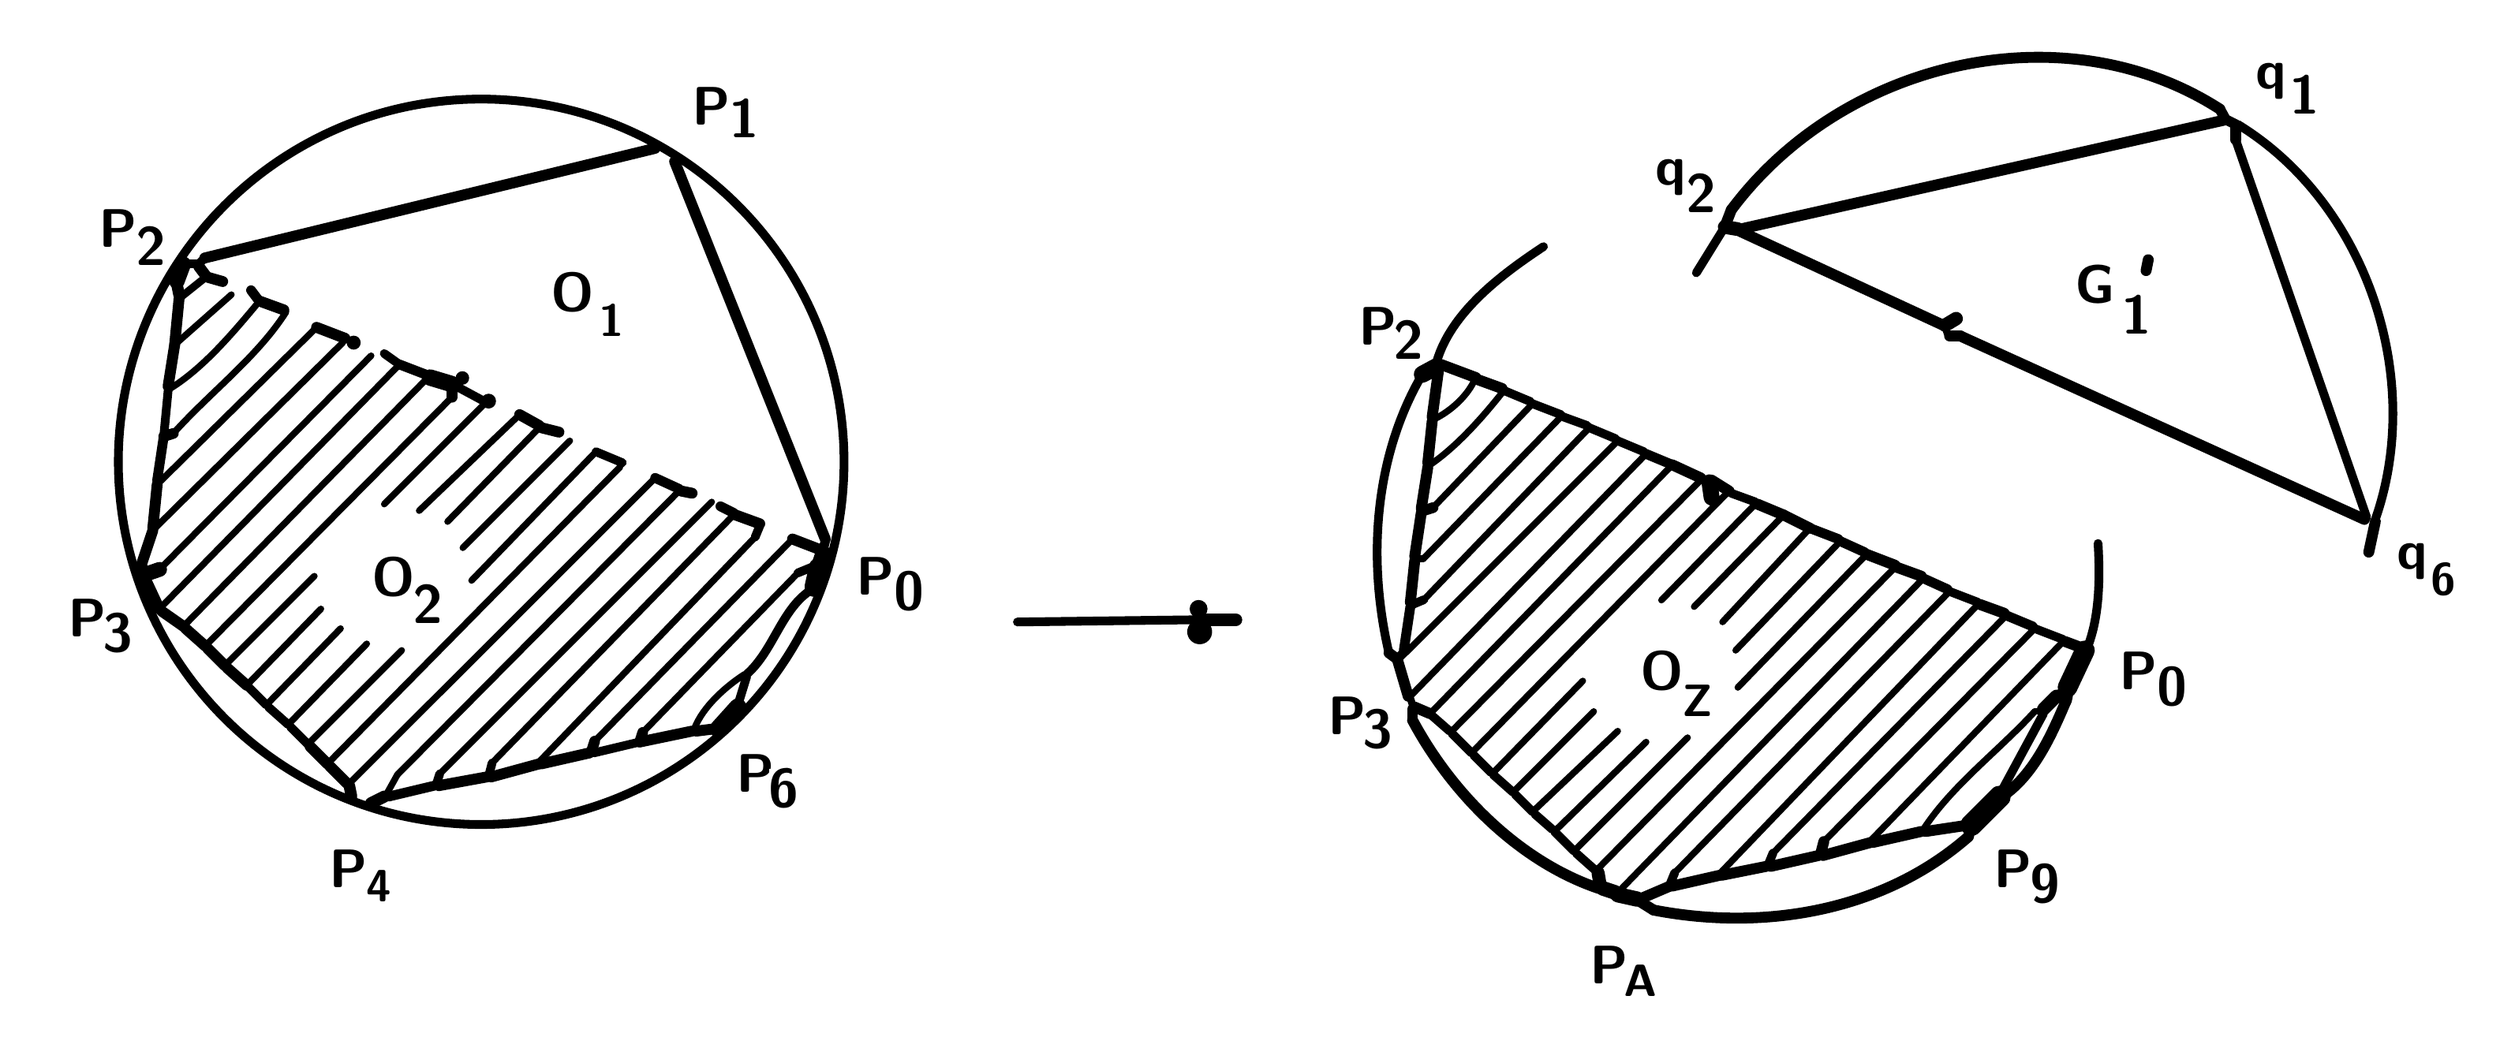
\begin{tikzpicture}[x=1pt, y=-1pt, line width=4.0pt, line cap=round, line join=round]

  %% ════ 填充区（prims2 的 fills）════

  %% ════ 直线段（prims2 的 strokes）════
  \draw[line width=4.0pt] (655.0,326.0) -- (664.0,335.0);
  \draw[line width=3.0pt] (202.0,241.0) -- (251.0,192.0);
  \draw[line width=5.0pt] (302.0,215.0) -- (307.0,216.0);
  \draw[line width=5.0pt] (787.0,96.0) -- (880.0,139.0);
  \draw[line width=6.7pt] (724.0,397.0) -- (730.0,399.0);
  \draw[line width=5.0pt] (149.0,349.0) -- (141.0,341.0);
  \draw[line width=5.0pt] (353.0,237.0) -- (366.0,242.0);
  \draw[line width=3.0pt] (646.0,316.0) -- (756.0,203.0);
  \draw[line width=5.0pt] (755.0,396.0) -- (741.0,402.0);
  \draw[line width=4.0pt] (456.0,275.0) -- (537.0,274.0);
  \draw[line width=5.0pt] (636.0,266.0) -- (638.0,247.0);
  \draw[line width=5.0pt] (780.0,94.0) -- (783.0,86.2);
  \draw[line width=4.8pt] (1006.8,40.0) -- (1009.0,44.0);
  \draw[line width=4.0pt] (780.0,94.0) -- (767.0,115.0);
  \draw[line width=6.3pt] (780.0,94.0) -- (786.0,95.0);
  \draw[line width=5.0pt] (72.0,127.0) -- (70.0,148.0);
  \draw[line width=3.0pt] (731.0,325.0) -- (693.0,361.0);
  \draw[line width=4.0pt] (794.0,220.0) -- (783.0,216.0);
  \draw[line width=4.0pt] (123.0,323.0) -- (131.0,331.0);
  \draw[line width=3.0pt] (684.0,352.0) -- (720.0,316.0);
  \draw[line width=3.0pt] (785.0,288.0) -- (832.0,239.0);
  \draw[line width=3.0pt] (75.0,276.0) -- (186.0,163.0);
  \draw[line width=5.0pt] (779.0,391.0) -- (799.0,387.0);
  \draw[line width=5.0pt] (649.0,159.0) -- (646.0,181.0);
  \draw[line width=4.0pt] (906.0,354.0) -- (926.0,317.0);
  \draw[line width=5.0pt] (936.0,284.0) -- (944.0,287.0);
  \draw[line width=3.0pt] (113.0,312.0) -- (146.0,278.0);
  \draw[line width=3.0pt] (908.0,273.0) -- (802.1,380.9);
  \draw[line width=4.0pt] (802.1,380.9) -- (800.0,386.0);
  \draw[line width=3.0pt] (715.0,302.0) -- (674.0,344.0);
  \draw[line width=9.0pt] (363.0,259.0) -- (365.0,250.0);
  \draw[line width=4.0pt] (896.0,266.0) -- (883.0,261.0);
  \draw[line width=3.0pt] (274.0,204.0) -- (141.0,339.0);
  \draw[line width=4.0pt] (122.0,322.0) -- (113.0,314.0);
  \draw[line width=4.9pt] (642.0,224.0) -- (646.4,222.6);
  \draw[line width=3.0pt] (646.4,222.6) -- (691.0,176.0);
  \draw[line width=3.0pt] (639.0,246.0) -- (642.0,246.0);
  \draw[line width=3.0pt] (642.0,246.0) -- (704.0,182.0);
  \draw[line width=3.0pt] (137.0,269.0) -- (104.0,303.0);
  \draw[line width=4.0pt] (730.0,191.0) -- (718.0,186.0);
  \draw[line width=4.0pt] (701.0,370.0) -- (693.0,363.0);
  \draw[line width=3.8pt] (936.0,306.0) -- (933.0,308.0);
  \draw[line width=3.0pt] (195.0,229.0) -- (236.0,187.0);
  \draw[line width=3.0pt] (857.0,251.0) -- (722.0,388.0);
  \draw[line width=5.0pt] (883.0,144.0) -- (888.0,144.0);
  \draw[line width=5.0pt] (888.0,144.0) -- (1073.0,228.0);
  \draw[line width=5.0pt] (638.0,314.0) -- (645.0,317.0);
  \draw[line width=6.7pt] (367.0,243.0) -- (365.0,249.0);
  \draw[line width=4.9pt] (283.0,330.0) -- (284.4,325.6);
  \draw[line width=3.0pt] (284.4,325.6) -- (355.5,252.5);
  \draw[line width=4.0pt] (355.5,252.5) -- (364.0,249.0);
  \draw[line width=4.0pt] (283.0,330.0) -- (262.0,335.0);
  \draw[line width=5.0pt] (283.0,330.0) -- (307.0,325.0);
  \draw[line width=5.0pt] (55.0,248.0) -- (60.0,233.0);
  \draw[line width=4.3pt] (55.0,248.0) -- (56.0,252.0);
  \draw[line width=5.0pt] (778.0,391.0) -- (756.0,396.0);
  \draw[line width=5.0pt] (238.0,186.0) -- (246.0,188.0);
  \draw[line width=5.0pt] (641.0,223.0) -- (644.0,204.0);
  \draw[line width=4.0pt] (679.0,169.0) -- (691.0,174.0);
  \draw[line width=5.0pt] (823.0,382.0) -- (801.0,387.0);
  \draw[line width=3.3pt] (881.0,140.0) -- (882.0,143.0);
  \draw[line width=3.0pt] (61.0,232.0) -- (147.0,147.0);
  \draw[line width=4.5pt] (832.0,237.0) -- (819.0,232.0);
  \draw[line width=4.5pt] (168.0,355.0) -- (189.0,350.0);
  \draw[line width=4.0pt] (692.0,362.0) -- (684.0,354.0);
  \draw[line width=3.0pt] (211.0,176.0) -- (166.0,221.0);
  \draw[line width=5.0pt] (213.0,346.0) -- (191.0,350.0);
  \draw[line width=10.0pt] (893.0,368.0) -- (906.0,355.0);
  \draw[line width=8.0pt] (319.0,324.0) -- (328.0,314.0);
  \draw[line width=3.0pt] (85.0,285.0) -- (197.0,172.0);
  \draw[line width=5.0pt] (197.0,172.0) -- (197.0,167.0);
  \draw[line width=3.0pt] (182.0,224.0) -- (228.0,180.0);
  \draw[line width=5.0pt] (228.0,180.0) -- (237.0,185.0);
  \draw[line width=3.0pt] (96.0,125.0) -- (70.0,148.0);
  \draw[line width=5.0pt] (60.0,232.0) -- (62.0,212.0);
  \draw[line width=5.0pt] (859.0,250.0) -- (870.0,254.0);
  \draw[line width=3.0pt] (731.0,399.0) -- (870.0,256.0);
  \draw[line width=6.0pt] (932.0,309.0) -- (926.0,315.0);
  \draw[line width=5.0pt] (819.0,232.0) -- (807.0,226.0);
  \draw[line width=3.0pt] (819.0,232.0) -- (779.0,275.0);
  \draw[line width=5.0pt] (63.0,269.0) -- (56.0,254.0);
  \draw[line width=3.0pt] (744.0,330.0) -- (703.0,370.0);
  \draw[line width=5.0pt] (64.0,270.0) -- (74.0,277.0);
  \draw[line width=4.0pt] (665.0,336.0) -- (673.0,344.0);
  \draw[line width=5.0pt] (870.0,371.0) -- (848.0,376.0);
  \draw[line width=5.0pt] (892.0,368.0) -- (872.0,371.0);
  \draw[line width=5.0pt] (93.0,295.0) -- (85.0,287.0);
  \draw[line width=5.0pt] (1078.0,229.0) -- (1075.0,243.0);
  \draw[line width=5.0pt] (94.0,296.0) -- (103.0,304.0);
  \draw[line width=5.0pt] (70.0,148.0) -- (67.0,167.0);
  \draw[line width=7.3pt] (773.0,211.0) -- (774.0,218.0);
  \draw[line width=7.0pt] (740.0,402.0) -- (731.0,400.0);
  \draw[line width=5.3pt] (150.0,350.0) -- (151.0,355.0);
  \draw[line width=4.0pt] (173.0,157.0) -- (166.0,152.0);
  \draw[line width=4.5pt] (173.0,157.0) -- (186.0,162.0);
  \draw[line width=3.0pt] (173.0,157.0) -- (64.0,268.0);
  \draw[line width=4.0pt] (190.0,349.0) -- (191.4,344.6);
  \draw[line width=3.0pt] (191.4,344.6) -- (316.0,220.0);
  \draw[line width=4.3pt] (368.0,238.0) -- (367.0,242.0);
  \draw[line width=3.0pt] (921.0,279.0) -- (825.4,375.6);
  \draw[line width=5.0pt] (825.4,375.6) -- (824.0,381.0);
  \draw[line width=4.0pt] (212.0,174.0) -- (199.0,167.0);
  \draw[line width=3.0pt] (655.0,325.0) -- (769.0,210.0);
  \draw[line width=5.3pt] (72.0,125.0) -- (71.0,120.0);
  \draw[line width=6.2pt] (886.0,136.0) -- (881.0,139.0);
  \draw[line width=5.0pt] (897.0,267.0) -- (908.0,271.0);
  \draw[line width=3.0pt] (123.0,321.0) -- (158.0,285.0);
  \draw[line width=5.0pt] (132.0,332.0) -- (140.0,340.0);
  \draw[line width=5.0pt] (299.0,64.0) -- (368.0,237.0);
  \draw[line width=4.5pt] (108.0,127.0) -- (105.0,123.0);
  \draw[line width=5.0pt] (795.0,221.0) -- (807.0,226.0);
  \draw[line width=3.0pt] (262.0,198.0) -- (206.0,256.0);
  \draw[line width=3.0pt] (174.0,288.0) -- (132.0,330.0);
  \draw[line width=4.7pt] (1014.0,47.0) -- (1010.0,45.0);
  \draw[line width=3.0pt] (325.0,227.0) -- (215.4,339.6);
  \draw[line width=4.0pt] (215.4,339.6) -- (214.0,345.0);
  \draw[line width=4.0pt] (702.0,371.0) -- (711.0,380.0);
  \draw[line width=5.0pt] (238.0,340.0) -- (260.0,335.0);
  \draw[line width=6.0pt] (540.0,274.0) -- (556.0,274.0);
  \draw[line width=5.0pt] (148.0,145.0) -- (135.0,140.0);
  \draw[line width=3.0pt] (135.0,140.0) -- (63.0,211.0);
  \draw[line width=4.5pt] (636.0,268.0) -- (633.0,288.0);
  \draw[line width=4.0pt] (692.0,175.0) -- (705.0,180.0);
  \draw[line width=3.0pt] (763.0,328.0) -- (712.0,379.0);
  \draw[line width=3.0pt] (743.0,199.0) -- (636.0,309.0);
  \draw[line width=5.0pt] (646.0,183.0) -- (644.0,202.0);
  \draw[line width=4.0pt] (731.0,192.0) -- (743.0,197.0);
  \draw[line width=3.0pt] (237.0,339.0) -- (335.9,236.1);
  \draw[line width=4.0pt] (335.9,236.1) -- (338.0,231.0);
  \draw[line width=3.0pt] (794.0,221.0) -- (751.0,265.0);
  \draw[line width=4.9pt] (893.0,369.0) -- (891.6,373.4);
  \draw[line width=5.0pt] (747.4,407.0) -- (741.0,403.0);
  \draw[line width=5.1pt] (84.0,116.0) -- (81.0,112.0);
  \draw[line width=4.0pt] (1074.0,227.0) -- (1014.0,54.0);
  \draw[line width=5.0pt] (1014.0,54.0) -- (1014.0,48.0);
  \draw[line width=4.5pt] (833.0,238.0) -- (844.0,243.0);
  \draw[line width=3.0pt] (847.0,375.0) -- (934.0,285.0);
  \draw[line width=7.5pt] (197.0,166.0) -- (187.0,163.0);
  \draw[line width=4.0pt] (81.0,111.0) -- (83.8,108.2);
  \draw[line width=5.0pt] (83.8,108.2) -- (290.0,58.0);
  \draw[line width=5.0pt] (637.0,320.0) -- (637.0,315.0);
  \draw[line width=4.0pt] (328.0,313.0) -- (332.0,300.0);
  \draw[line width=3.0pt] (922.0,316.0) -- (925.0,316.0);
  \draw[line width=6.8pt] (57.0,253.0) -- (63.1,250.9);
  \draw[line width=3.0pt] (63.1,250.9) -- (160.0,153.0);
  \draw[line width=4.0pt] (104.0,305.0) -- (112.0,313.0);
  \draw[line width=9.0pt] (945.0,288.0) -- (937.0,305.0);
  \draw[line width=3.0pt] (94.0,294.0) -- (134.0,254.0);
  \draw[line width=7.0pt] (71.0,119.0) -- (74.0,111.0);
  \draw[line width=4.0pt] (683.0,353.0) -- (674.0,345.0);
  \draw[line width=4.0pt] (76.0,111.0) -- (80.0,111.0);
  \draw[line width=4.9pt] (261.0,334.0) -- (262.4,329.6);
  \draw[line width=3.0pt] (262.4,329.6) -- (352.0,238.0);
  \draw[line width=4.5pt] (871.0,255.0) -- (882.0,260.0);
  \draw[line width=3.0pt] (781.0,216.0) -- (665.0,334.0);
  \draw[line width=3.0pt] (844.0,245.0) -- (786.0,305.0);
  \draw[line width=5.0pt] (769.0,209.0) -- (756.0,203.0);
  \draw[line width=3.5pt] (83.0,118.0) -- (73.0,126.0);
  \draw[line width=4.0pt] (67.0,169.0) -- (65.0,190.0);
  \draw[line width=4.5pt] (921.0,277.0) -- (909.0,272.0);
  \draw[line width=4.5pt] (320.0,222.0) -- (326.0,225.0);
  \draw[line width=4.0pt] (706.0,181.0) -- (717.0,185.0);
  \draw[line width=5.0pt] (666.0,163.0) -- (650.0,157.0);
  \draw[line width=3.0pt] (634.0,289.0) -- (730.0,193.0);
  \draw[line width=3.0pt] (882.0,262.0) -- (757.1,389.9);
  \draw[line width=4.0pt] (757.1,389.9) -- (755.0,395.0);
  \draw[line width=3.0pt] (717.0,187.0) -- (642.2,264.8);
  \draw[line width=4.0pt] (642.2,264.8) -- (637.0,267.0);
  \draw[line width=5.0pt] (327.0,226.0) -- (338.0,230.0);
  \draw[line width=4.5pt] (744.0,198.0) -- (756.0,203.0);
  \draw[line width=3.0pt] (150.0,349.0) -- (290.1,209.0);
  \draw[line width=4.5pt] (290.1,209.0) -- (301.0,214.0);
  \draw[line width=4.0pt] (263.0,197.0) -- (275.0,202.0);
  \draw[line width=4.5pt] (62.0,210.0) -- (65.0,190.0);
  \draw[line width=5.5pt] (166.0,355.0) -- (160.0,358.0);
  \draw[line width=4.0pt] (712.0,381.0) -- (721.0,389.0);
  \draw[line width=5.0pt] (120.0,132.0) -- (109.0,128.0);
  \draw[line width=3.0pt] (807.0,226.0) -- (766.0,268.0);
  \draw[line width=5.0pt] (317.0,324.0) -- (309.0,325.0);
  \draw[line width=5.0pt] (825.0,382.0) -- (847.0,376.0);
  \draw[line width=5.0pt] (215.0,346.0) -- (237.0,340.0);
  \draw[line width=6.0pt] (937.0,306.0) -- (936.0,311.0);
  \draw[line width=3.0pt] (778.0,390.0) -- (895.0,268.0);
  \draw[line width=4.9pt] (630.0,292.0) -- (626.2,289.2);
  \draw[line width=7.8pt] (641.5,161.5) -- (648.0,158.0);
  \draw[line width=4.2pt] (630.0,292.0) -- (633.0,289.0);
  \draw[line width=5.0pt] (630.0,292.0) -- (635.0,309.0);
  \draw[line width=5.0pt] (1009.0,45.0) -- (787.0,95.0);
  \draw[line width=4.0pt] (654.0,325.0) -- (646.0,318.0);
  \draw[line width=5.0pt] (782.0,215.0) -- (774.0,210.0);
  \draw[line width=5.0pt] (75.0,278.0) -- (84.0,286.0);
  \draw[line width=6.0pt] (723.0,396.0) -- (722.0,390.0);
  \draw[line width=5.0pt] (845.0,244.0) -- (858.0,249.0);
  \draw[line width=5.0pt] (973.0,114.0) -- (974.0,109.0);
  \draw[line width=4.9pt] (65.0,190.0) -- (69.4,188.6);
  \draw[line width=4.0pt] (935.0,283.0) -- (922.0,278.0);
  \draw[line width=5.0pt] (85.0,117.0) -- (92.0,119.0);
  \draw[line width=5.0pt] (678.0,168.0) -- (667.0,164.0);
  \draw[line width=5.0pt] (638.0,245.0) -- (641.0,225.0);
  \draw[line width=3.4pt] (636.0,310.0) -- (637.0,313.0);
  \draw[line width=3.0pt] (167.0,354.0) -- (172.0,345.0);
  \draw[line width=3.0pt] (172.0,345.0) -- (300.0,216.0);

  %% ════ 曲线（prims2 的 curves —— 三段式，坐标同为 (y,x)）════
  \draw[line width=5.0pt] (783.0,86.2) .. controls (834.0,17.7) and (935.3,-6.0) .. (1006.8,40.0);
  \draw[line width=3.0pt] (68.0,168.0) .. controls (83.1,158.7) and (96.8,142.4) .. (108.0,129.0);
  \draw[line width=4.0pt] (946.0,287.0) .. controls (951.8,272.6) and (951.9,254.5) .. (951.0,239.0);
  \draw[line width=5.0pt] (907.0,355.0) .. controls (921.4,345.3) and (929.5,327.2) .. (936.0,312.0);
  \draw[line width=4.0pt] (332.0,299.0) .. controls (344.6,287.9) and (347.9,268.7) .. (362.0,260.0);
  \draw[line width=3.0pt] (331.0,299.0) .. controls (322.1,304.8) and (311.8,314.0) .. (308.0,324.0);
  \draw[line width=5.0pt] (891.6,373.4) .. controls (852.6,407.6) and (798.0,416.8) .. (747.4,407.0);
  \draw[line width=5.0pt] (722.0,397.0) .. controls (685.8,384.6) and (655.0,353.7) .. (637.0,320.0);
  \draw[line width=3.0pt] (871.0,370.0) .. controls (884.2,349.8) and (904.9,334.6) .. (922.0,316.0);
  \draw[line width=3.0pt] (678.0,170.0) .. controls (669.1,181.2) and (657.3,194.6) .. (645.0,203.0);
  \draw[line width=3.0pt] (647.0,182.0) .. controls (654.1,178.6) and (661.4,172.1) .. (665.0,165.0);
  \draw[line width=4.0pt] (626.2,289.2) .. controls (616.2,246.5) and (619.4,199.2) .. (641.5,161.5);
  \draw[line width=3.0pt] (69.4,188.6) .. controls (85.8,170.2) and (107.9,153.6) .. (121.0,133.0);
  \draw[line width=4.0pt] (697.0,103.0) .. controls (677.5,115.9) and (654.5,133.2) .. (648.0,156.0);
  \draw[line width=4.0pt] (1078.0,228.0) .. controls (1100.6,163.4) and (1074.3,83.3) .. (1015.0,47.0);

  %% ════ 圆 / 椭圆（probe 精测）════
  \draw (210.4,201.6) circle (166.2);

  %% ════ 实心点 ════
  \fill (152.0,147.0) circle (3.2);
  \fill (201.8,163.2) circle (3.1);
  \fill (213.8,173.8) circle (3.4);
  \fill (539.0,269.0) circle (4.1);
  \fill (539.5,279.5) circle (5.7);

  %% ════ 标签（probe 直接给的 \node 行）════
  %% ⚠ 全部补了 fill=white：文字在最上层，否则与曲线交叉干扰
     \node[anchor=center,inner sep=0pt,fill=white,font=\fontsize{32.0}{40.0}\selectfont] at (1030.1,27.4) {\textsf{\textbf{\textit{q}}}};   % box(1020,14,18,23)
     \node[anchor=center,inner sep=0pt,fill=white,font=\fontsize{23.7}{29.7}\selectfont] at (1045.8,33.4) {\textsf{\textbf{1}}};   % box(1039,25,8,16)
     \node[anchor=center,inner sep=0pt,fill=white,font=\fontsize{29.8}{37.3}\selectfont] at (316.0,38.5) {\textsf{\textbf{\textit{P}}}};   % box(305,26,18,23)
     \node[anchor=center,inner sep=0pt,fill=white,font=\fontsize{23.7}{29.7}\selectfont] at (330.8,44.4) {\textsf{\textbf{1}}};   % box(324,36,8,16)
     \node[anchor=center,inner sep=0pt,fill=white,font=\fontsize{32.0}{40.0}\selectfont] at (755.1,71.4) {\textsf{\textbf{\textit{q}}}};   % box(745,58,18,23)
     \node[anchor=center,inner sep=0pt,fill=white,font=\fontsize{23.6}{29.6}\selectfont] at (769.1,78.9) {\textsf{\textbf{2}}};   % box(763,70,11,17)
     \node[anchor=center,inner sep=0pt,fill=white,font=\fontsize{29.8}{37.3}\selectfont] at (44.0,94.5) {\textsf{\textbf{\textit{P}}}};   % box(33,82,18,23)
     \node[anchor=center,inner sep=0pt,fill=white,font=\fontsize{23.6}{29.6}\selectfont] at (59.1,102.9) {\textsf{\textbf{2}}};   % box(53,94,11,17)
     \node[anchor=center,inner sep=0pt,fill=white,font=\fontsize{31.4}{39.2}\selectfont] at (949.7,120.3) {\textsf{\textbf{\textit{G}}}};   % box(939,108,22,23)
     \node[anchor=center,inner sep=0pt,fill=white,font=\fontsize{30.4}{38.0}\selectfont] at (252.3,124.0) {\textsf{\textbf{\textit{O}}}};   % box(240,112,22,22)
     \node[anchor=center,inner sep=0pt,fill=white,font=\fontsize{23.7}{29.7}\selectfont] at (968.8,134.4) {\textsf{\textbf{1}}};   % box(962,126,8,16)
     \node[anchor=center,inner sep=0pt,fill=white,font=\fontsize{29.8}{37.3}\selectfont] at (621.0,139.5) {\textsf{\textbf{\textit{P}}}};   % box(610,127,18,23)
     \node[anchor=center,inner sep=0pt,fill=white,font=\fontsize{21.5}{26.9}\selectfont] at (270.0,136.9) {\textsf{\textbf{1}}};   % box(264,129,7,15)
     \node[anchor=center,inner sep=0pt,fill=white,font=\fontsize{23.6}{29.6}\selectfont] at (635.1,145.9) {\textsf{\textbf{2}}};   % box(629,137,11,17)
     \node[anchor=center,inner sep=0pt,fill=white,font=\fontsize{32.0}{40.0}\selectfont] at (1095.1,247.4) {\textsf{\textbf{\textit{q}}}};   % box(1085,234,18,23)
     \node[anchor=center,inner sep=0pt,fill=white,font=\fontsize{31.0}{38.8}\selectfont] at (170.3,254.5) {\textsf{\textbf{\textit{O}}}};   % box(158,242,22,23)
     \node[anchor=center,inner sep=0pt,fill=white,font=\fontsize{29.2}{36.4}\selectfont] at (390.9,254.0) {\textsf{\textbf{\textit{P}}}};   % box(380,242,18,22)
     \node[anchor=center,inner sep=0pt,fill=white,font=\fontsize{22.7}{28.3}\selectfont] at (1109.1,255.6) {\textsf{\textbf{6}}};   % box(1103,247,11,16)
     \node[anchor=center,inner sep=0pt,fill=white,font=\fontsize{23.8}{29.8}\selectfont] at (406.5,260.7) {\textsf{\textbf{0}}};   % box(399,252,11,17)
     \node[anchor=center,inner sep=0pt,fill=white,font=\fontsize{23.6}{29.6}\selectfont] at (186.1,266.9) {\textsf{\textbf{2}}};   % box(180,258,11,17)
     \node[anchor=center,inner sep=0pt,fill=white,font=\fontsize{29.2}{36.4}\selectfont] at (29.9,273.0) {\textsf{\textbf{\textit{P}}}};   % box(19,261,18,22)
     \node[anchor=center,inner sep=0pt,fill=white,font=\fontsize{23.0}{28.7}\selectfont] at (43.9,280.1) {\textsf{\textbf{3}}};   % box(38,271,11,17)
     \node[anchor=center,inner sep=0pt,fill=white,font=\fontsize{31.0}{38.8}\selectfont] at (751.3,297.5) {\textsf{\textbf{\textit{O}}}};   % box(739,285,22,23)
     \node[anchor=center,inner sep=0pt,fill=white,font=\fontsize{30.6}{38.3}\selectfont] at (969.5,297.5) {\textsf{\textbf{\textit{P}}}};   % box(958,285,19,23)
     \node[anchor=center,inner sep=0pt,fill=white,font=\fontsize{24.9}{31.1}\selectfont] at (985.1,304.7) {\textsf{\textbf{0}}};   % box(977,296,12,17)
     \node[anchor=center,inner sep=0pt,fill=white,font=\fontsize{20.3}{25.4}\selectfont] at (767.7,311.2) {\textsf{\textbf{\textit{Z}}}};   % box(761,302,11,17)
     \node[anchor=center,inner sep=0pt,fill=white,font=\fontsize{29.2}{36.4}\selectfont] at (606.9,318.0) {\textsf{\textbf{\textit{P}}}};   % box(596,306,18,22)
     \node[anchor=center,inner sep=0pt,fill=white,font=\fontsize{23.0}{28.7}\selectfont] at (620.9,324.1) {\textsf{\textbf{3}}};   % box(615,315,11,17)
     \node[anchor=center,inner sep=0pt,fill=white,font=\fontsize{29.8}{37.3}\selectfont] at (336.0,344.5) {\textsf{\textbf{\textit{P}}}};   % box(325,332,18,23)
     \node[anchor=center,inner sep=0pt,fill=white,font=\fontsize{23.4}{29.2}\selectfont] at (349.1,351.1) {\textsf{\textbf{6}}};   % box(343,342,11,17)
     \node[anchor=center,inner sep=0pt,fill=white,font=\fontsize{30.0}{37.4}\selectfont] at (149.5,388.0) {\textsf{\textbf{\textit{P}}}};   % box(138,376,19,22)
     \node[anchor=center,inner sep=0pt,fill=white,font=\fontsize{29.2}{36.4}\selectfont] at (911.9,388.0) {\textsf{\textbf{\textit{P}}}};   % box(901,376,18,22)
     \node[anchor=center,inner sep=0pt,fill=white,font=\fontsize{23.4}{29.2}\selectfont] at (926.9,395.1) {\textsf{\textbf{9}}};   % box(920,386,11,17)
     \node[anchor=center,inner sep=0pt,fill=white,font=\fontsize{22.0}{27.6}\selectfont] at (163.7,395.9) {\textsf{\textbf{4}}};   % box(157,388,12,15)
     \node[anchor=center,inner sep=0pt,fill=white,font=\fontsize{29.2}{36.4}\selectfont] at (726.9,432.0) {\textsf{\textbf{\textit{P}}}};   % box(716,420,18,22)
     \node[anchor=center,inner sep=0pt,fill=white,font=\fontsize{19.2}{24.0}\selectfont] at (741.3,439.3) {\textsf{\textbf{\textit{A}}}};   % box(734,431,11,16)

  % 钉死画布：否则超出的图元/控制点会把页面撑大，1:1 回比就失准
  \pgfresetboundingbox
  \path[use as bounding box] (0,0) rectangle (1125,455);
\end{tikzpicture}
\end{document}

% ⚠ 待核清单（probe 拿不准，人眼过一遍）：
%   · 可疑字形：\node[anchor=center,inner sep=0pt,font=\fontsize{30.4}{38.0}\selectfont] at (252.3,124.0) {\textsf{\textbf{\te
%   · 可疑字形：\node[anchor=center,inner sep=0pt,font=\fontsize{31.0}{38.8}\selectfont] at (170.3,254.5) {\textsf{\textbf{\te
%   · 可疑字形：\node[anchor=center,inner sep=0pt,font=\fontsize{31.0}{38.8}\selectfont] at (751.3,297.5) {\textsf{\textbf{\te
%   · 未识别/跳过：⑤ 跳过/未识别的字形
